\documentclass[../index.tex]{subfiles}

\begin{document}

Так як головною метою цієї роботи є опис загального алгоритму для знаходження
найоптимальнішого шляху для обміну, ми спробуємо формалізувати визначення ваги у
графі \(G_{t} = (V_{t}, E_{t})\).

Розглянувши формулу обміну~\eqref{eq:swap} ми можемо побачити гіперболічну
залежність вкладів однієї валюти від іншої.

Чим більшим ми вкладаємо валюти \(X\) тим більшим стає його відношення із \(Y\),
тим самим чим більше існує валюти \(X\) тим менш вона ціна відносно \(Y\) за
мінімальну одиницю, тим самим AMM біржі балансують ціни.

\begin{figure}[h]
	\centering
	\begin{tikzpicture}

		\node (x) at (0, -1) {X};
		\node (y) at (4, 0) {Y};
		\node (z) at (8, 0) {Z};
		\node (w) at (4, -2) {W};

		\draw[->] (x) to node [above, sloped] {\(f_{X/Y}(x)\)} (y);
		\draw[->] (y) to node [above] {\(f_{Y/Z}(x)\)} (z);
		\draw[->] (x) to node [below,sloped] {\(f_{X/W}(x)\)} (w);

	\end{tikzpicture}
	\caption{Графічне представлення графу біржи}\label{fig:amm-graph}
\end{figure}

Більшість сучасних алгоритмів знаходження оптимального шляху між всіма парами
(all-to-all по класифікації~\cite{deo1980shortest}) потребують аби вага ребра
була дійсною функцією від двох вершин $f: (V, V) \to \mathbb{R}$, проте у нашому випадку
розглядаєма вага ребра залежить від теперішніх вкладів у вершини та об'єму
обміну. Спробуємо розглянути можливі випадки переведення нашої задачі до
стандартної із можливістю ``сумувати'' ваги, та порівнювати їх між собою.

\subsection{Обчислення ваги при фіксованому об'ємі}\label{sec:weight-non-fixed}

Зафіксуємо стан графу при деякому $t$, таким чином розміри вкладів у функції
обміну стають константами, проте об'єми обміну все ще є невідомим значенням.
Тому нехай для пари $X/Y$ зафіксуємо об'єм обміну як відоме $x$.

Таким чином всі функції обміну на будь-якому з можливих шляхів між $X$ та $Y$
обчислюються у дійсні значення з $\mathbb{R}^{+}$ за допомогою, наприклад,
~\eqref{eq:nth-swap}. Проте при обході графа утворенні значення неможна
порівнювати допоки шлях з $X$ в $Y$ не дійде докінця.

Нехай стан біржи на момент $t$ має вигляд як на~\ref{fig:eval-func-graph}. Для
знаходження ``найкоротшого'' шляху (у нашому випадку шляху при котрому ми за $X$
отримаємо якомога більше $Y$) у подібному графі здавалося б можна використати,
наприклад, алгоритм Дейкстри~\cite{dijkstra} так як на цей раз всі значення ваг
є просто числами. Проте, якщо розглянути $S_{X/W}$ та $S_{X/Z}$, то достатньо
легко зрозуміти, що значення об'єму цих обмінів не можна порівнювати так як вони
є зовсім різними валютами.

\begin{figure}[h]
	\centering
	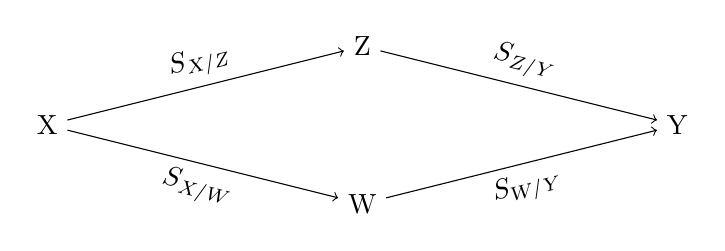
\begin{tikzpicture}

		\node (x) at (0, -1) {X};
		\node (z) at (4, 0) {Z};
		\node (y) at (8, -1) {Y};
		\node (w) at (4, -2) {W};

		\draw[->] (x) to node [above,sloped] {\(S_{X/Z}\)} (z);
		\draw[->] (z) to node [above,sloped] {\(S_{Z/Y}\)} (y);
		\draw[->] (x) to node [below,sloped] {\(S_{X/W}\)} (w);
		\draw[->] (w) to node [below,sloped] {\(S_{W/Y}\)} (y);

	\end{tikzpicture}
	\caption{Графічне представлення двох можливих шляхів обміну між $X$ та $Y$
		при фіксованому $x$. $S_{X/Y}$ --- це значення отримуємої валюти $Y$ за
		фіксонану кількість $x$ валюти $X$}\label{fig:eval-func-graph}
\end{figure}

Не рідко на біржах існує валюта до котрої можна перевести будь яку іншу на
платформі. Наприклад на фіатних біржах чи біржах ціних паперів --- це може бути
долар, а на криптобіржах нативна валюта мережі (ethereum, bitcoin).

\begin{lemma}
	Тому пропонується розглянути два припущення:

	\begin{itemize}
		\item Якщо в такій ситуації існує пара обміну між $W$ та $Z$, то через неї
		      ми можемо привести номінал одного значення в інший аби порівняти
		      значення.
		\item Якщо на біржі присутня ``базова'' валюта, до котрої можна перевести
		      будь-яку іншу, то можна перевести обидві валюти в одну ``базову'' для
		      порівняння.
	\end{itemize}
\end{lemma}

Таким чином послідовність дій для порівняння ребер можна описати
алгоритмом~\ref{alg:cap}. Приклад графу після алгортму є
рисунок~\ref{fig:eval-func-graph-base}.

\begin{algorithm}
\caption{Алгоритм знаходження ваги ребра}\label{alg:cap}
\begin{algorithmic}
\Function{swap}{$\Delta x$, $X$, $Y$} \Comment{Об'єм обміну між вершинами $X$ та $Y$}
\EndFunction{}
\Function{choose}{$X$} \Comment{Вибрати як наступний шлях обміну $X$}
\EndFunction{}
\Ensure{$V_{t}$} \Comment{множина вершин графа}
\Ensure{$E_{t}$} \Comment{множина ребер}
\Ensure{$v_{i+1} \in V_{t}$} \Comment{перша вершина через котру проходить шлях}
\Ensure{$v_{j+1} \in V_{t}$} \Comment{друга вершина з котрою порівнюється шлях}
\Ensure{$v_{base} \in V_{t}$} \Comment{вершина базової валюти біржі}
\Require{$\Delta x > 0$}
\State{$volume_{left} \gets 0$}
\State{$volume_{right} \gets 0$}
\If{$(v_{i+1}, v_{j+1}) \in  E_{t}$}
	\State{$volume_{tmp} \gets \Call{swap}{\Delta x, v_{i}, v_{i+1}}$}
  	\State{$volume_{left} \gets \Call{swap}{volume_{tmp}, v_{i+1}, v_{j+1}}$}
	\State{$volume_{right} \gets \Call{swap}{\Delta x, v_{j}, v_{j+1}}$}
  \ElsIf{$(v_{base}, v_{i+1}) \in E_{t} \land (v_{base}, v_{j+1}) \in E_{t}$ }
	\State{$volume_{left} \gets \Call{swap}{\Delta x, v_{base}, v_{i+1}}$}
	\State{$volume_{right} \gets \Call{swap}{\Delta x, v_{base}, v_{j+1}}$}
  \EndIf{}
  \If{$volume_{left} < volume_{right}$}
	$\Call{choose}{v_{j+1}}$
  \Else{}
	$\Call{choose}{v_{i+1}}$
  \EndIf{}
\end{algorithmic}
\end{algorithm}

\begin{figure}[h]
	\centering
	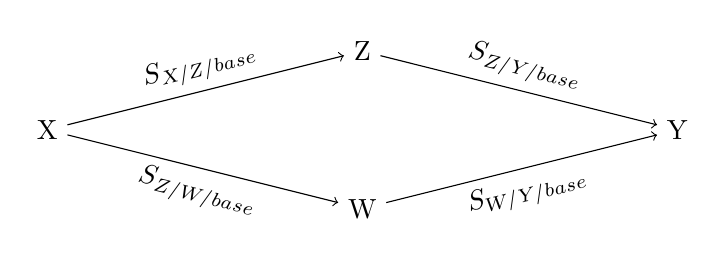
\begin{tikzpicture}

		\node (x) at (0, -1) {X};
		\node (z) at (4, 0) {Z};
		\node (y) at (8, -1) {Y};
		\node (w) at (4, -2) {W};

		\draw[->] (x) to node [above,sloped] {\(S_{X/Z/base}\)} (z);
		\draw[->] (z) to node [above,sloped] {\(S_{Z/Y/base}\)} (y);
		\draw[->] (x) to node [below,sloped] {\(S_{Z/W/base}\)} (w);
		\draw[->] (w) to node [below,sloped] {\(S_{W/Y/base}\)} (y);

	\end{tikzpicture}
	\caption{\label{fig:eval-func-graph-base} Графічне представлення двох можливих
	  шляхів обміну між $X$ та $Y$ при фіксованому $x$. $S_{base}$ --- значення
	  отримуєме при обміні що переведенне до базовох валюти}
\end{figure}

Для переведення задачі до стандартної для використання алгоритмів обходу графа
достатньо за вагу обчислити різницю минулого отриманого значення і теперішнього
(рис.~\ref{fig:eval-func-graph-weight}). Тобто, якщо $S_{i}$ --- об'єми призведені
до базових на шляху між валютами, то ваги будуть:

\begin{equation*}
W_{i} = S_{i} - S_{i-1}, S_{0} = 0
\end{equation*}

\begin{figure}[h]
	\centering
	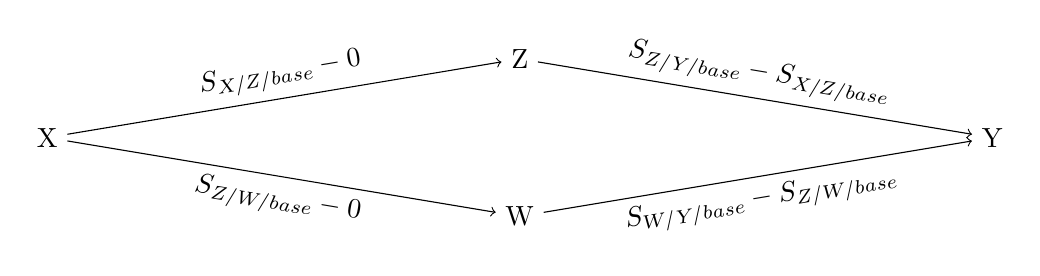
\begin{tikzpicture}

		\node (x) at (-2, -1) {X};
		\node (z) at (4, 0) {Z};
		\node (y) at (10, -1) {Y};
		\node (w) at (4, -2) {W};

		\draw[->] (x) to node [above,sloped] {\(S_{X/Z/base} - 0\)} (z);
		\draw[->] (z) to node [above,sloped] {\(S_{Z/Y/base} - S_{X/Z/base}\)} (y);
		\draw[->] (x) to node [below,sloped] {\(S_{Z/W/base} - 0\)} (w);
		\draw[->] (w) to node [below,sloped] {\(S_{W/Y/base} - S_{Z/W/base}\)} (y);

	\end{tikzpicture}
	\caption{\label{fig:eval-func-graph-weight} Графічне представлення двох
	  можливих шляхів обміну між $X$ та $Y$ при фіксованому $x$ після
	  переведення задачі до стандартної}
\end{figure}

\subsection{Спрощення графа при нефіксованому об'ємі}

При нефіксованому об'ємі спробуємо розглянути преоптимізації графа, що
допоможуть спросити пошук при невідомому $\Delta x$.

Розглянемо два шляхи, котрі утворилися при обході графа:

\begin{equation*}
 \begin{aligned}
   C_{0} \implies \ldots \implies C_{j} \\
   C_{0} \implies \ldots \implies C_{i}
 \end{aligned}
\end{equation*}

Обидва вони починаються з однієї вершини та закінчуються на відмінних, проте як
і в розділі~\ref{sec:weight-non-fixed}, доповнимо шляхи переведенням до базової
вершини:

\begin{equation*}
 \begin{aligned}
   C_{0} \implies \ldots \implies C_{j} \implies C_{base}\\
   C_{0} \implies \ldots \implies C_{i} \implies C_{base}
 \end{aligned}
\end{equation*}

При не фіксованому об'ємі функція обміну залишається залежною від $x$ і
оперувати конкретними значеннями для сумування ваги шляхів ми не можемо. Проте з
розділів~\ref{sec:func-composition}~та~\ref{sec:nth-swap} відомо, що композиція
функцій обміну по шляху утворює функцію обміну між початковою та кінцевою
вершиною:

\begin{equation*}
 \begin{aligned}
   (f_{C_{0}/C_{1}} \circ \ldots f_{C_{j}/C_{base}})(x) = f_{C_{0}/C_{base}}^{1}(x)\\
   (f_{C_{0}/C_{1}} \circ \ldots f_{C_{i}/C_{base}})(x) = f_{C_{0}/C_{base}}^{2}(x)
 \end{aligned}
\end{equation*}

З розділу~\ref{sec:swap-graph} відомо, що для таких функцій з резервами
$R_{\Omega}, R_{\Xi}, R'_{\Omega}, R'_{\Xi}$ утворених аналогічно до заміни
з~\eqref{eq:swap-omega-xi} можливо розглянути три випадки.

\begin{enumerate}
  \item $R_{\Xi} = R'_{\Xi}$ та $R_{\Omega} = R'_{\Omega} \implies f_{1} = f_{2}$ --- варто
		залишити обидва шляхи і переходити на наступні вершини.
  \item $R_{\Xi} = R'_{\Xi}$ та $R_{\Omega} \neq R'_{\Omega}$ --- криві мають перетин лише у
		$x = 0$, тобто
		$\forall x > 0 \, f_{C_{0}/C_{base}}^{1}(x) > f_{C_{0}/C_{base}}^{2}(x)$ або
		$\forall x > 0 \, f_{C_{0}/C_{base}}^{2}(x) > f_{C_{0}/C_{base}}^{1}(x)$. Варто
		залишити лише один з шляхів що є завжди більшим.
  \item $R_{\Xi} \neq R'_{\Xi}$ та $R_{\Omega} \neq R'_{\Omega}$ --- варто залишити обидва шляхи,
		враховуючи, що при $\Delta x > x_{2}$ кращим є шлях через $C_{i}$ (або
		$C_{j}$).
\end{enumerate}

У третьому випадку при обході можуть утворюватися такі точки перетину кривих
$\exists x_{2}, x'_{2}$, що $\left(0, x_{2}\right) \cap{} \left(x'_{2}, \infty{} \right) = \emptyset$,
і з обмеженнями з розділу~\ref{sec:weight-non-fixed}, утворюються несумісні
умови при котрих лише одна наступна вершина є правильною, або жодна. Завдяки
чому можна спростити граф позбувшися таких шляхів при котрих обмін неможливий
взагалі через відсутніть ліквідності в парах.

У випадках коли $x_{2} > R_{X}$ $x_{2}$ --- можна знехтувати і вважати що одна з
функцій завжди більше або меньша за іншу (як в другому випадку).
\end{document}
